\begin{frame}{Local Features: Detect, Describe, Match}
  \begin{columns}[T,onlytextwidth]
    \column{0.52\textwidth}
      \begin{itemize}\footnotesize\itemsep0.3em
        \item \textbf{Detect} repeatable points: the same corner or blob is found again from another viewpoint.
        \item \textbf{Describe} each point by a vector computed from its neighbourhood, built to change little under rotation, scale and illumination. \textbf{Match} by nearest neighbour in descriptor space.
        \item \textbf{SIFT} (Scale Invariant Feature Transform; Lowe, 2004): keypoints are extrema of a difference-of-Gaussians scale space (differences of successively blurred copies of the image). The descriptor holds gradient-orientation histograms over $4\times4$ cells $\times$ 8 bins $=128$ values, measured relative to the keypoint's dominant orientation.
        \item \textbf{ORB} (Oriented FAST and Rotated BRIEF; Rublee et al., 2011): FAST corners (an intensity test on a ring of pixels) given an orientation, and a 256-bit string of pixel-pair intensity comparisons rotated with the keypoint, compared by Hamming distance (the number of differing bits). On the same 640$\times$480 images with about 1000 features: 15.3\,ms per frame against 5228.7\,ms for SIFT.
      \end{itemize}
    \column{0.46\textwidth}
      \centering
      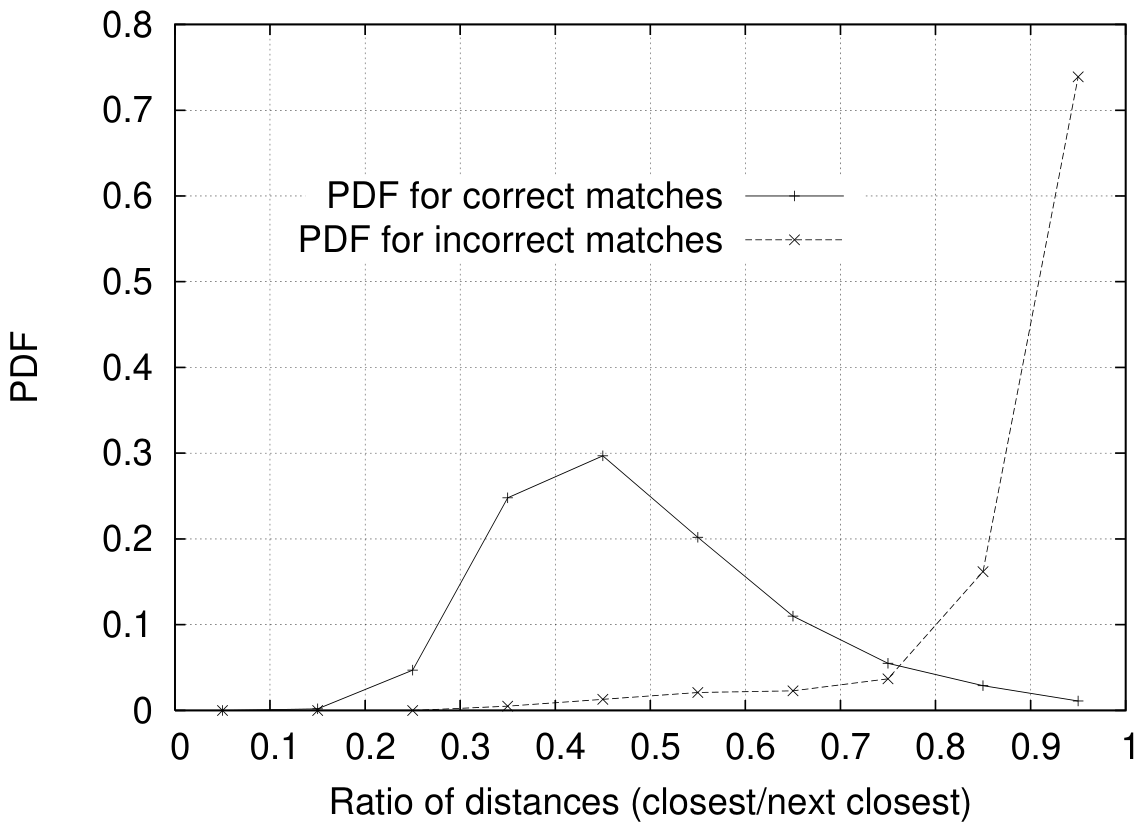
\includegraphics[width=\linewidth,height=0.40\textheight,keepaspectratio]{images/3d-vision/sift_fig11_distance_ratio_pdf.png}\\[0.2em]
      {\scriptsize Lowe, ``Distinctive Image Features from Scale-Invariant Keypoints,'' IJCV 60(2), 2004, \href{https://doi.org/10.1023/B:VISI.0000029664.99615.94}{doi:10.1023/B:VISI.0000029664.99615.94}, Figure~11.\par}
      \vspace{0.5em}
      \raggedright\footnotesize
      \textbf{Ratio test:} keep the nearest neighbour only if $d_1/d_2<0.8$, where $d_1$ and $d_2$ are the distances to the closest and second-closest descriptors. Correct matches (solid curve) have low ratios; Lowe reports that the 0.8 threshold ``eliminates 90\% of the false matches while discarding less than 5\% of the correct matches.''
  \end{columns}
\end{frame}

\begin{frame}{Learned Detectors and Matchers}
  \begin{columns}[T,onlytextwidth]
    \column{0.56\textwidth}
      \begin{itemize}\scriptsize\itemsep0.3em
        \item \textbf{SuperPoint} (DeTone et al., 2018): one fully convolutional network, a shared encoder with two heads (keypoint heatmap, 256-D descriptors), run once per image. Self-supervised: a detector trained on rendered synthetic shapes with known corners labels real images by \emph{homographic adaptation}, pooling its detections over many random homographic warps of each image.
        \item \textbf{SuperGlue} (covered earlier) matches two keypoint sets jointly with self- and cross-attention and a Sinkhorn assignment.
        \item \textbf{LightGlue} (Lindenberger et al., 2023) adapts its computation to the pair. After each layer it predicts how confident each point is, stops once enough points are confident (depth), and drops points it is sure are unmatchable (width). For pose estimation on MegaDepth-1500 (1500 outdoor image pairs): 31.4\,ms per pair against 70.0\,ms for SuperGlue, at similar accuracy.
        \item \textbf{LoFTR} (Local Feature TRansformer; Sun et al., 2021) has no detector. Self- and cross-attention over a dense grid of 1/8-resolution features give coarse matches (mutual nearest neighbours), each refined to sub-pixel in a window of 1/2-resolution features. It finds matches on texture-less walls, where detectors struggle to find repeatable points.
        \item \textbf{RoMa} (Edstedt et al., 2024): dense matching, a warp plus a certainty for every pixel, from frozen DINOv2 coarse features (covered earlier) and ConvNet fine features.
      \end{itemize}
    \column{0.42\textwidth}
      \centering
      \vspace{0.8em}
      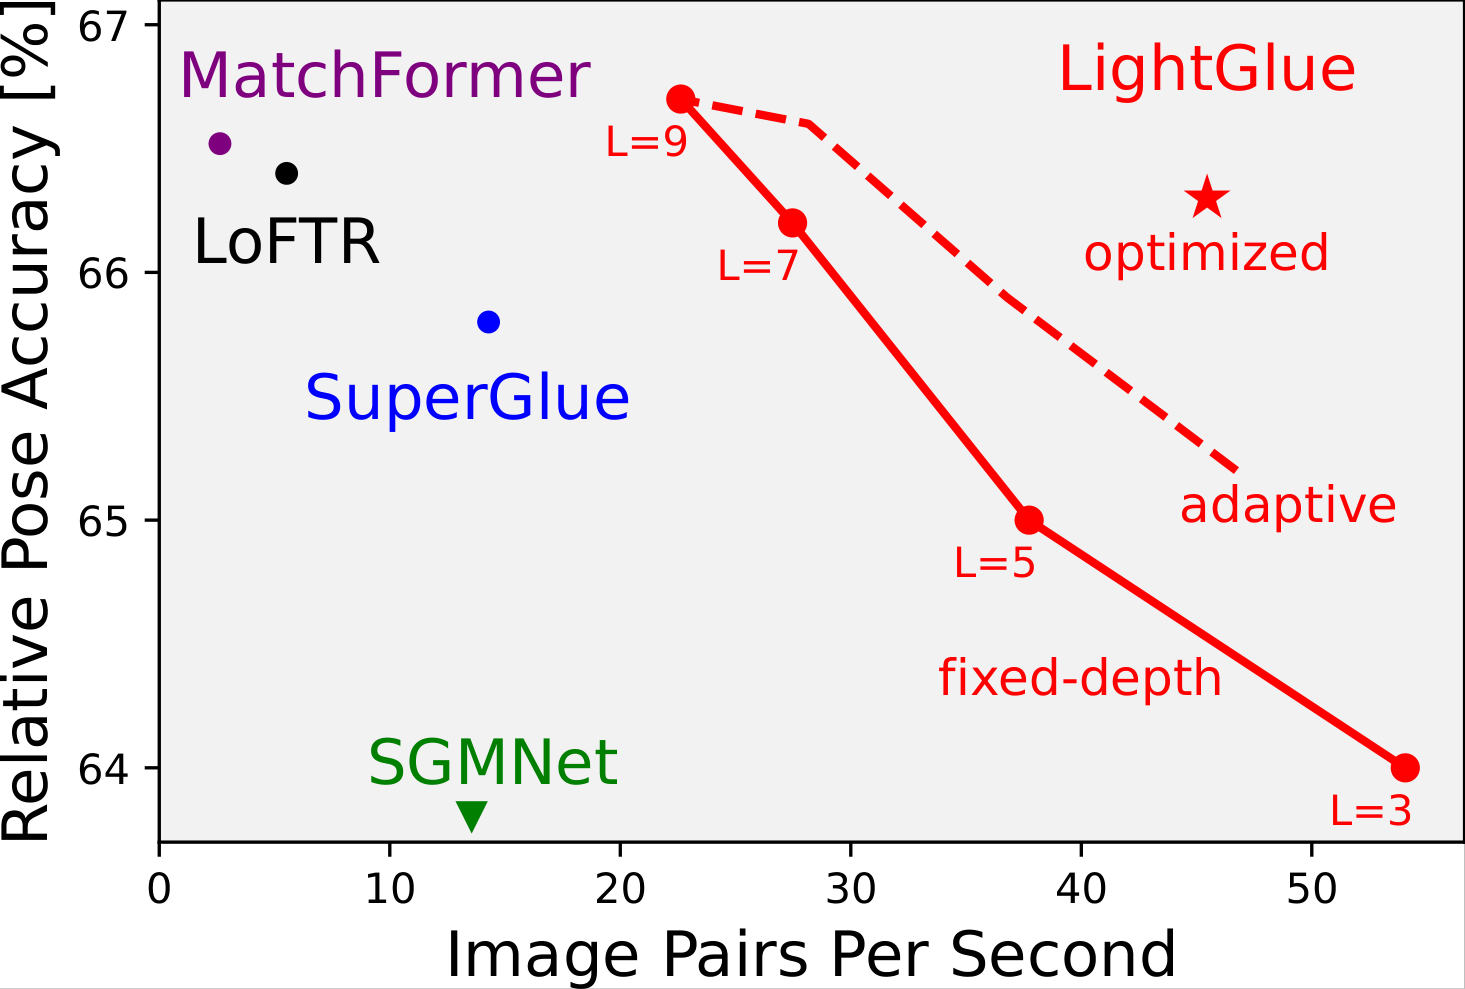
\includegraphics[width=\linewidth,height=0.55\textheight,keepaspectratio]{images/3d-vision/lightglue_fig1_speed_accuracy.png}\\[0.2em]
      {\scriptsize ``LightGlue matches sparse features faster and better than existing approaches like SuperGlue.'' Lindenberger et al., ``LightGlue: Local Feature Matching at Light Speed,'' ICCV 2023, \href{https://arxiv.org/abs/2306.13643v1}{arXiv:2306.13643v1}, Figure~1.\par}
  \end{columns}
\end{frame}

\begin{frame}{Epipolar Geometry}
  \begin{columns}[T,onlytextwidth]
    \column{0.58\textwidth}
      \centering
      % Exact 3D construction in an orthographic view (45 deg elevation): cameras toed in by
      % 45 deg, focal distance 1, image planes 2.5 x 1.1. Epipoles and image points are computed
      % ray-plane intersections, so they lie on their planes, rays and epipolar lines.
      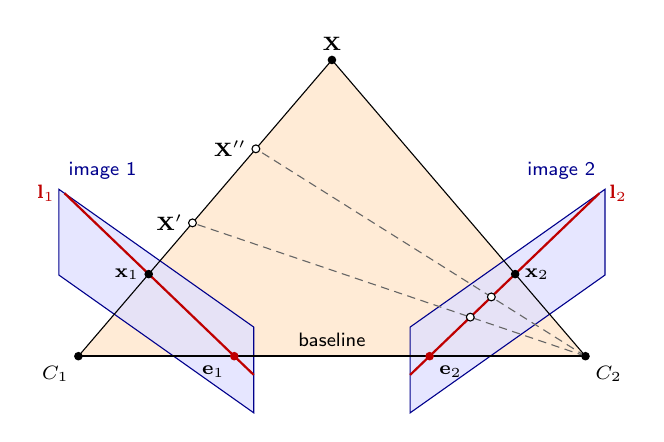
\begin{tikzpicture}[font=\sffamily\scriptsize, >=latex,
          x={(1.4cm,0cm)}, y={(0cm,0.99cm)}, z={(0cm,0.99cm)},
          pt/.style={circle, fill=black, inner sep=1.1pt},
          cand/.style={circle, draw=black, fill=white, inner sep=1.0pt},
          epi/.style={red!75!black, thick},
          imgplane/.style={draw=blue!55!black, fill=blue!12, fill opacity=0.8}]
        \coordinate (C1) at (0,0,0);
        \coordinate (C2) at (4.6,0,0);
        \coordinate (X) at (2.3,1,2.8);
        \coordinate (Xa) at (1.035,0.45,1.26);
        \coordinate (Xb) at (1.61,0.7,1.96);
        \coordinate (e1) at (1.414,0,0);
        \coordinate (e2) at (3.186,0,0);
        \coordinate (x1) at (0.638,0.277,0.776);
        \coordinate (x2) at (3.962,0.277,0.776);
        \coordinate (x2a) at (3.555,0.132,0.369);
        \coordinate (x2b) at (3.746,0.2,0.56);
        \fill[orange!16] (C1) -- (X) -- (C2) -- cycle;
        \filldraw[imgplane] (-0.177,-0.55,1.591) -- (1.591,-0.55,-0.177) -- (1.591,0.55,-0.177) -- (-0.177,0.55,1.591) -- cycle;
        \filldraw[imgplane] (3.009,-0.55,-0.177) -- (4.777,-0.55,1.591) -- (4.777,0.55,1.591) -- (3.009,0.55,-0.177) -- cycle;
        \draw[thick] (C1) -- (C2);
        \draw (C1) -- (X);
        \draw (C2) -- (X);
        \draw[densely dashed, black!60] (C2) -- (Xa);
        \draw[densely dashed, black!60] (C2) -- (Xb);
        \draw[epi] (1.591,-0.063,-0.177) -- (-0.126,0.55,1.54);
        \draw[epi] (3.009,-0.063,-0.177) -- (4.726,0.55,1.54);
        \node[pt] at (C1) {};
        \node[pt] at (C2) {};
        \node[pt] at (X) {};
        \node[cand] at (Xa) {};
        \node[cand] at (Xb) {};
        \node[pt, fill=red!75!black] at (e1) {};
        \node[pt, fill=red!75!black] at (e2) {};
        \node[pt] at (x1) {};
        \node[pt] at (x2) {};
        \node[cand] at (x2a) {};
        \node[cand] at (x2b) {};
        \node[below left] at (C1) {$C_1$};
        \node[below right] at (C2) {$C_2$};
        \node[above] at (2.3,0,0) {baseline};
        \node[above] at (X) {$\mathbf{X}$};
        \node[left] at (Xa) {$\mathbf{X}'$};
        \node[left] at (Xb) {$\mathbf{X}''$};
        \node[left] at (x1) {$\mathbf{x}_1$};
        \node[right] at (x2) {$\mathbf{x}_2$};
        \node[below left] at (e1) {$\mathbf{e}_1$};
        \node[below right] at (e2) {$\mathbf{e}_2$};
        \node[left, red!75!black] at (-0.126,0.55,1.54) {$\mathbf{l}_1$};
        \node[right, red!75!black] at (4.726,0.55,1.54) {$\mathbf{l}_2$};
        \node[anchor=south west, blue!55!black] at (-0.177,0.55,1.591) {image 1};
        \node[anchor=south east, blue!55!black] at (4.777,0.55,1.591) {image 2};
      \end{tikzpicture}
    \column{0.40\textwidth}
      \begin{itemize}\footnotesize\itemsep0.35em
        \item The baseline (defined above) joins the camera centres $C_1$ and $C_2$. Together with a scene point $\mathbf{X}$ it spans the \textbf{epipolar plane} (shaded).
        \item The \textbf{epipoles} $\mathbf{e}_1,\mathbf{e}_2$ are where the baseline pierces the image planes: $\mathbf{e}_2$ is the image of $C_1$ in view 2, and $\mathbf{e}_1$ the image of $C_2$ in view 1.
        \item The epipolar plane cuts the image planes in the \textbf{epipolar lines} $\mathbf{l}_1,\mathbf{l}_2$. Every point on the ray through $\mathbf{x}_1$ ($\mathbf{X}$, $\mathbf{X}'$, $\mathbf{X}''$) lies in that plane, so its image in view 2 lies on $\mathbf{l}_2$.
        \item The search for the match of $\mathbf{x}_1$ shrinks from the whole image (2D) to the line $\mathbf{l}_2$ (1D). All epipolar lines of an image pass through its epipole.
      \end{itemize}
  \end{columns}
\end{frame}

\begin{frame}{The Essential and Fundamental Matrices}
  \begin{columns}[T,onlytextwidth]
    \column{0.52\textwidth}
      \begin{itemize}\footnotesize\itemsep0.3em
        \item Take camera 1 as the world frame: a point at $\mathbf{X}_1$ in camera 1 is at $\mathbf{X}_2=R\,\mathbf{X}_1+\mathbf{t}$ in camera 2, so $\mathbf{t}$ is the position of $C_1$ seen from $C_2$.
        \item The normalized coordinates (defined above), written homogeneously as $\hat{\mathbf{x}}_i=K_i^{-1}\tilde{\mathbf{x}}_i=(x_i,y_i,1)^\top$, are ray directions: $\mathbf{X}_i=Z_i\,\hat{\mathbf{x}}_i$, with $Z_i$ the depth in camera $i$.
        \item In camera-2 axes, $\hat{\mathbf{x}}_2$, $\mathbf{t}$ and $R\hat{\mathbf{x}}_1$ all lie in the epipolar plane, so they are coplanar: $\hat{\mathbf{x}}_2\cdot(\mathbf{t}\times R\hat{\mathbf{x}}_1)=0$, that is
        \[ \hat{\mathbf{x}}_2^\top E\,\hat{\mathbf{x}}_1=0,\qquad E=[\mathbf{t}]_\times R, \]
        with the cross-product matrix $[\mathbf{t}]_\times=\left[\begin{smallmatrix}0&-t_3&t_2\\ t_3&0&-t_1\\ -t_2&t_1&0\end{smallmatrix}\right]$, so that $[\mathbf{t}]_\times\mathbf{a}=\mathbf{t}\times\mathbf{a}$ for any vector $\mathbf{a}$.
        \item Substituting $\hat{\mathbf{x}}_i=K_i^{-1}\tilde{\mathbf{x}}_i$ moves the constraint to pixels: $\tilde{\mathbf{x}}_2^\top F\,\tilde{\mathbf{x}}_1=0$ with $F=K_2^{-\top}E\,K_1^{-1}$.
      \end{itemize}
    \column{0.46\textwidth}
      \centering
      {\footnotesize\setlength{\tabcolsep}{3pt}
      \begin{tabular}{@{}>{\raggedright\arraybackslash}p{1.55cm} >{\raggedright\arraybackslash}p{2.2cm} >{\raggedright\arraybackslash}p{2.2cm}@{}}
        \toprule
         & \textbf{Essential} $E$ & \textbf{Fundamental} $F$ \\
        \midrule
        Points & normalized $\hat{\mathbf{x}}$ ($K$ known) & pixels $\tilde{\mathbf{x}}$ \\
        \addlinespace[0.3em]
        Degrees of freedom & 5: 3 for $R$, 3 for $\mathbf{t}$, minus 1 for scale & 7: 9 entries, minus 1 for scale, minus 1 for $\det F=0$ \\
        \addlinespace[0.3em]
        Rank & 2, singular values $(\sigma,\sigma,0)$ & 2 \\
        \bottomrule
      \end{tabular}\par}
      \vspace{0.4em}
      \begin{itemize}\footnotesize\itemsep0.3em
        \item \textbf{Epipolar line} of $\tilde{\mathbf{x}}_1$ in image 2: $\mathbf{l}_2=F\tilde{\mathbf{x}}_1$, so its match satisfies $\tilde{\mathbf{x}}_2^\top\mathbf{l}_2=0$.
        \item \textbf{Epipoles} are the null vectors: $F\mathbf{e}_1=\mathbf{0}$ and $F^\top\mathbf{e}_2=\mathbf{0}$.
      \end{itemize}
  \end{columns}
  \vspace{0.3em}
  {\scriptsize Hartley and Zisserman, \emph{Multiple View Geometry in Computer Vision}, 2nd ed., 2004, \href{https://doi.org/10.1017/CBO9780511811685}{doi:10.1017/CBO9780511811685}, Table~9.1 and Section~9.6.\par}
\end{frame}

\begin{frame}{Estimating F: The Eight-Point Algorithm}
  \begin{columns}[T,onlytextwidth]
    \column{0.50\textwidth}
      \begin{itemize}\footnotesize\itemsep0.3em
        \item A match $(u_1,v_1)\leftrightarrow(u_2,v_2)$ turns $\tilde{\mathbf{x}}_2^\top F\tilde{\mathbf{x}}_1=0$ into one linear equation in the 9 entries $\mathbf{f}=(F_{11},F_{12},\dots,F_{33})^\top$:
        \[ (u_2u_1,\ u_2v_1,\ u_2,\ v_2u_1,\ v_2v_1,\ v_2,\ u_1,\ v_1,\ 1)\,\mathbf{f}=0. \]
        \item Stack $n\geq8$ matches into $A\mathbf{f}=\mathbf{0}$, with $A$ of size $n\times9$. The minimizer of $\lVert A\mathbf{f}\rVert$ subject to $\lVert\mathbf{f}\rVert=1$ is the right singular vector of $A$ for its smallest singular value.
        \item \textbf{Enforce rank 2:} from $F=U\,\mathrm{diag}(\sigma_1,\sigma_2,\sigma_3)\,V^\top$ keep $U\,\mathrm{diag}(\sigma_1,\sigma_2,0)\,V^\top$, the closest singular matrix in Frobenius norm (root of the sum of squared entries). Without it the epipolar lines do not meet in a single epipole.
      \end{itemize}
      \vspace{0.3em}
      {\scriptsize Hartley, ``In Defense of the Eight-Point Algorithm,'' TPAMI 19(6), 1997, \href{https://doi.org/10.1109/34.601246}{doi:10.1109/34.601246}. Nist\'er, ``An Efficient Solution to the Five-Point Relative Pose Problem,'' TPAMI 26(6), 2004, \href{https://doi.org/10.1109/TPAMI.2004.17}{doi:10.1109/TPAMI.2004.17}.\par}
    \column{0.48\textwidth}
      \begin{itemize}\footnotesize\itemsep0.3em
        \item \textbf{Normalize first} (Hartley, 1997), with translate-and-scale matrices $T_i$ as for the homography DLT: estimate $\hat{F}$ from the points $T_i\tilde{\mathbf{x}}_i$, then undo it: $F=T_2^\top\hat{F}\,T_1$.
        \item \textbf{Why:} with pixel coordinates near 100, a row of $A$ mixes entries near $10^4$ with entries equal to 1, so $A^\top A$ has entries from $10^8$ down to 1 and a condition number (eigenvalue ratio) of at least about $10^4$. Small noise then swings the solution; after normalization the linear algorithm is comparable with the best iterative ones.
        \item \textbf{Minimal solvers:} 7 matches leave a 2-D null space, $F=\alpha F_1+(1-\alpha)F_2$, and $\det F=0$ is a cubic in $\alpha$: up to 3 solutions. With $K$ known, 5 matches fix $E$ (Nist\'er, 2004) as roots of a tenth-degree polynomial: up to 10 solutions.
      \end{itemize}
  \end{columns}
\end{frame}

\begin{frame}{RANSAC: Fitting Despite Outliers}
  \begin{columns}[T,onlytextwidth]
    \column{0.48\textwidth}
      {\footnotesize \textbf{RANSAC} (random sample consensus; Fischler and Bolles, 1981) repeats $N$ times:\par}
      \begin{enumerate}\footnotesize\itemsep0.15em
        \item Sample a minimal set of $s$ matches at random.
        \item Fit the model to them: four-point homography, five-point $E$, seven- or eight-point $F$.
        \item Count the \textbf{inliers}: matches whose error is below a threshold $\tau$ (for $F$, the distance from $\tilde{\mathbf{x}}_2$ to its epipolar line $F\tilde{\mathbf{x}}_1$).
        \item Keep the model with the most inliers.
      \end{enumerate}
      {\footnotesize Finally, refit the best model on all of its inliers.\par}
      \begin{itemize}\footnotesize\itemsep0.2em
        \item With inlier ratio $w$, a sample is outlier-free with probability $w^s$, and all $N$ samples fail with probability $(1-w^s)^N$. Asking for success probability $p$:
      \end{itemize}
      \[ N=\frac{\log(1-p)}{\log(1-w^s)} \]
    \column{0.50\textwidth}
      \centering
      {\footnotesize Samples $N$ for $p=0.99$ (rounded up)\par}
      \vspace{0.3em}
      {\footnotesize\setlength{\tabcolsep}{4pt}
      \begin{tabular}{@{}lrrrr@{}}
        \toprule
         & $s=4$ & $s=5$ & $s=7$ & $s=8$ \\
         & $H$ & $E$ & $F$ & $F$ \\
        \midrule
        $w=0.5$ & 72 & 146 & 588 & 1177 \\
        $w=0.3$ & 567 & 1893 & 21\,055 & 70\,188 \\
        \bottomrule
      \end{tabular}\par}
      \vspace{0.6em}
      \begin{itemize}\footnotesize\itemsep0.3em
        \item $N$ grows exponentially with the sample size $s$. At 30\% inliers the eight-point algorithm needs about 37 times as many samples as the five-point solver (70\,188 against 1893).
        \item This is why minimal solvers matter: they shrink $s$ inside the exponent.
      \end{itemize}
      \vspace{0.2em}
      {\scriptsize Fischler and Bolles, ``Random Sample Consensus: A Paradigm for Model Fitting with Applications to Image Analysis and Automated Cartography,'' \emph{Communications of the ACM} 24(6), 1981, \href{https://doi.org/10.1145/358669.358692}{doi:10.1145/358669.358692}, which derives the same number of trials.\par}
  \end{columns}
\end{frame}

\begin{frame}{Relative Pose and Triangulation}
  \begin{columns}[T,onlytextwidth]
    \column{0.56\textwidth}
      \begin{itemize}\footnotesize\itemsep0.3em
        \item \textbf{Four candidates.} Take the SVD $E=U\,\mathrm{diag}(1,1,0)\,V^\top$ with $\det U=\det V=1$. Then
        \[ R\in\{UWV^\top,\ UW^\top V^\top\},\qquad \mathbf{t}=\pm\mathbf{u}_3, \]
        with $W=\left[\begin{smallmatrix}0&-1&0\\ 1&0&0\\ 0&0&1\end{smallmatrix}\right]$ and $\mathbf{u}_3$ the last column of $U$.
        \item \textbf{Cheirality} (a point must lie in front of a camera): triangulate a match with each candidate; only one puts it at positive depth in both views.
        \item \textbf{Scale:} $E$ is defined only up to scale (any multiple of $E$ satisfies $\hat{\mathbf{x}}_2^\top E\,\hat{\mathbf{x}}_1=0$), so the length of $\mathbf{t}$ is not observable and is set to $\lVert\mathbf{t}\rVert=1$. Metric scale needs outside information, such as a known length.
        \item \textbf{Triangulation (DLT):} $\tilde{\mathbf{x}}\times P\tilde{\mathbf{X}}=\mathbf{0}$ gives two independent equations per view, $u\,\mathbf{p}^{3\top}\tilde{\mathbf{X}}-\mathbf{p}^{1\top}\tilde{\mathbf{X}}=0$ and $v\,\mathbf{p}^{3\top}\tilde{\mathbf{X}}-\mathbf{p}^{2\top}\tilde{\mathbf{X}}=0$, with $\mathbf{p}^{k\top}$ row $k$ of $P$. Stack both views into a $4\times4$ system, take the SVD null vector, then refine $\mathbf{X}$ by minimizing the reprojection error.
      \end{itemize}
    \column{0.42\textwidth}
      \centering
      % Exact geometry: point at depth 3, ray error +-3 deg; the red regions are the computed
      % intersections of the two error wedges (depth extent 2.84 for baseline 0.8, 0.69 for 4).
      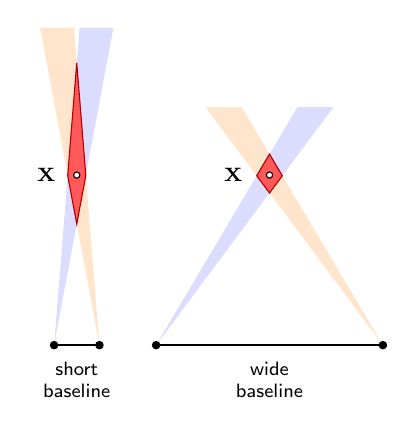
\begin{tikzpicture}[font=\sffamily\scriptsize, >=latex, x=0.72cm, y=0.72cm,
          cam/.style={circle, fill=black, inner sep=1.1pt},
          wedgeone/.style={fill=blue!30, fill opacity=0.45},
          wedgetwo/.style={fill=orange!45, fill opacity=0.45},
          region/.style={fill=red!65, draw=red!70!black}]
        \fill[wedgeone] (-0.4,0) -- (0.05,5.6) -- (0.647,5.6) -- cycle;
        \fill[wedgetwo] (0.4,0) -- (-0.647,5.6) -- (-0.05,5.6) -- cycle;
        \filldraw[region] (0,2.138) -- (0.16,2.992) -- (0,4.977) -- (-0.16,2.992) -- cycle;
        \draw[thick] (-0.4,0) -- (0.4,0);
        \node[cam] at (-0.4,0) {};
        \node[cam] at (0.4,0) {};
        \node[below, align=center] at (0,-0.12) {short\\baseline};
        \fill[wedgeone] (1.4,0) -- (3.893,4.2) -- (4.529,4.2) -- cycle;
        \fill[wedgetwo] (5.4,0) -- (2.271,4.2) -- (2.907,4.2) -- cycle;
        \filldraw[region] (3.4,2.684) -- (3.626,2.988) -- (3.4,3.37) -- (3.174,2.988) -- cycle;
        \draw[thick] (1.4,0) -- (5.4,0);
        \node[cam] at (1.4,0) {};
        \node[cam] at (5.4,0) {};
        \node[below, align=center] at (3.4,-0.12) {wide\\baseline};
        \node[cam, fill=white, draw=black, inner sep=0.8pt] at (0,3) {};
        \node[cam, fill=white, draw=black, inner sep=0.8pt] at (3.4,3) {};
        \node[left] at (-0.2,3) {$\mathbf{X}$};
        \node[left] at (3.1,3) {$\mathbf{X}$};
      \end{tikzpicture}\\[0.3em]
      {\scriptsize\raggedright Both cameras see $\mathbf{X}$ (white dot) with the same $\pm3^\circ$ ray error. With nearly parallel rays (short baseline, little parallax) the possible positions (red) stretch about four times as far in depth.\par}
  \end{columns}
\end{frame}
